\section{Model}

\begin{figure*}[t]
\begin{center}
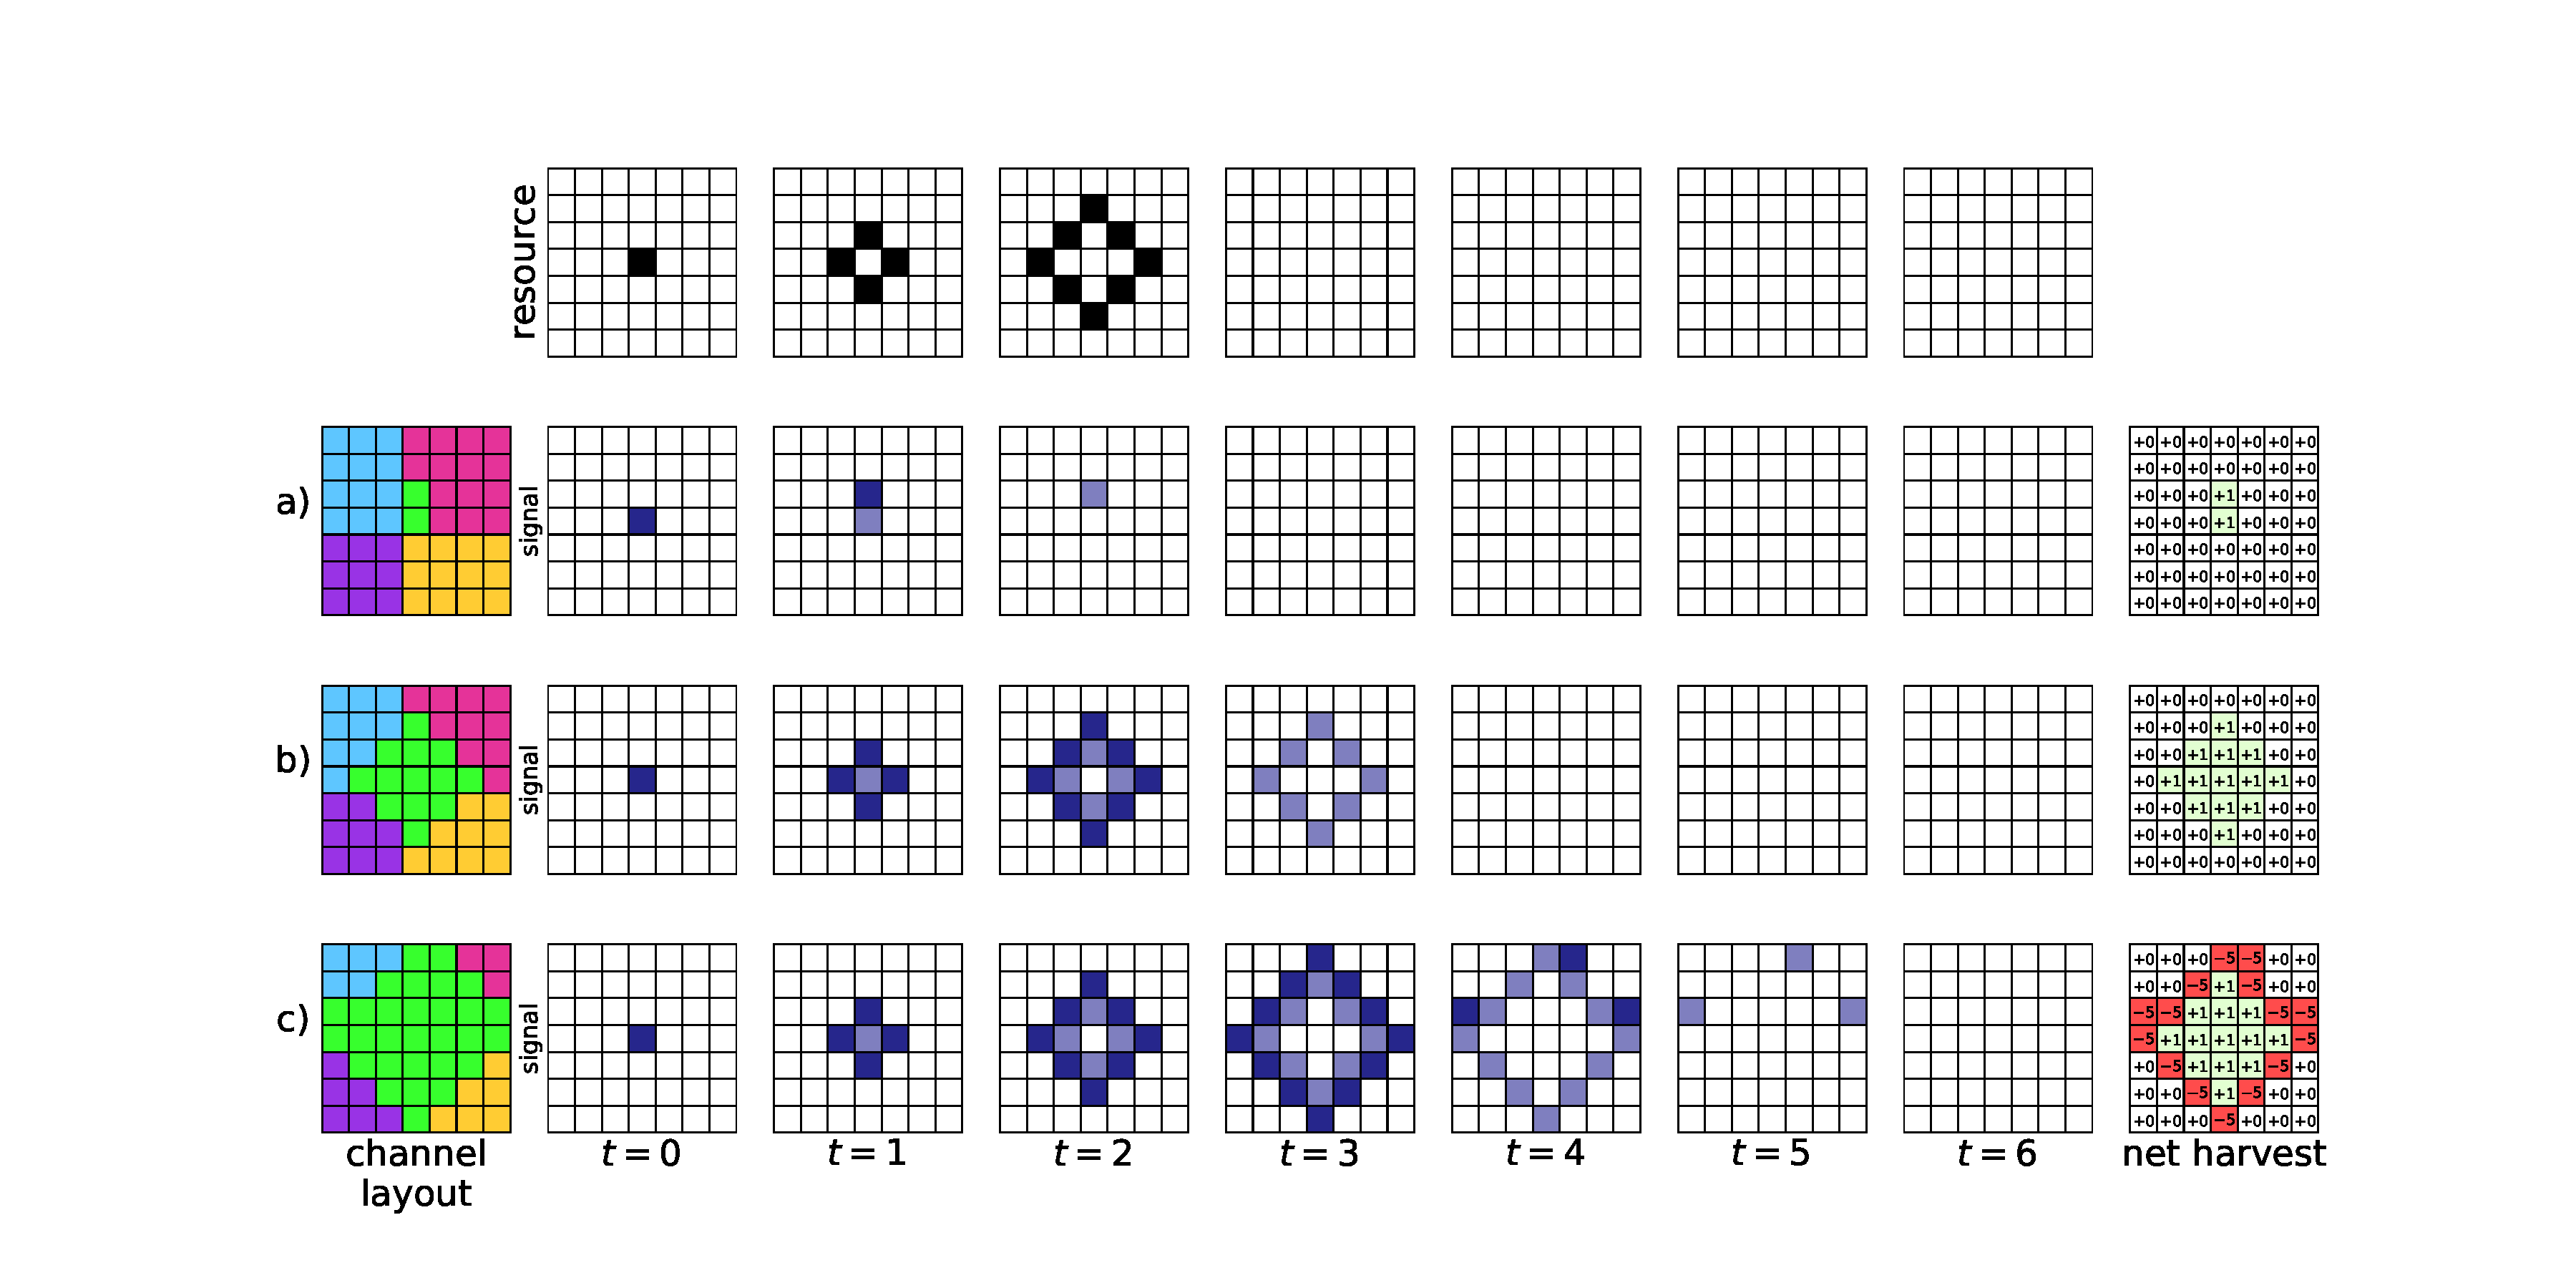
\includegraphics[width=\textwidth,trim={4cm 0.5cm 4cm 0.5cm},clip]{img/explanatory}
\caption{
\textbf{Activation signaling, and net resource collection for three different-sized same-channel networks during a resource wave event.}
At the top, a resource wave is depicted propagating over three updates and then ceasing for four updates (left to right).
In row $a$, a small two-cell channel-signaling group (far left, in green) is activated; tracking the resource wave (top) yields a small net resource harvest (far right).
In row $b$, an intermediate-sized 13-cell channel-signaling group yields a high net resource harvest.
Finally, in row $c$, a large 29-cell channel-signaling group incurs a net negative resource harvest.
In rows $a$, $b$, and $c$, dark purple indicates the active state, light purple indicates the quiescent state, and white indicates the ready state.
}
\label{fig:explanatory}
\end{center}
\end{figure*}


In previous work \cite{moreno2018toward}, we introduced the DISHTINY (DIStributed Hierarchical Transitions in IndividualitY) model, which seeks to achieve the evolution of transitions in individuality by explicitly registering organisms in cooperating groups that coordinate spatiotemporally to maximize the harvest of a resource.
Detection of such a transition in DISHTINY is accomplished by identifying resource-sharing and reproductive division of labor among organisms registered to the same cooperating group.
We designed this system such that hierarchal transitions across an arbitrary number of levels of individuality can be selected for and meaningfully detected.
Furthermore, DISHTINY is decentralized and amenable to massive parallelization via distributed computing.
We believe that such scalability is an essential consideration in the pursuit of artificial systems capable of generating complexity and novelty rivaling that of biological life via open-ended evolution \cite{ackley2011pursue, ackley2016indefinite}.

DISHTINY allows cell-like organisms to replicate across a toroidal grid.
Over discrete timesteps (``updates''), the cells can collect a continuous-valued resource.
Once sufficient resource has been accrued, cells may spend resource to place a daughter cell on an adjoining tile of the toroidal grid (i.e., reproduce), replacing any existing cell already there.
As cells reproduce, they can choose to include offspring in the parent's cooperating ``signaling channel'' group or force offspring to create a new cooperating ``signaling channel'' group.

As shown at the top of Figure \ref{fig:explanatory}, resources appear at a single point then spread outwards update-by-update in a diamond-shaped wave, disappearing when the expanding wave reaches a predefined limit.
Cells must be in a costly ``activated'' state to collect resource as it passes.
The cell at the starting position of a resource wave is automatically activated, and will send the activate signal to neighboring cells on the same signaling channel.
The newly activated cells, in turn, activate their own neighbors registered to the same signaling channel.
Neighbors registered to other signaling channels do not activate.
Each cell, after sending the activation signal, enters a temporary quiescent state so as not to reactivate from the signal.
In this manner, cells sharing a signaling channel activate in concert with the expanding resource wave.
As shown Figure \ref{fig:explanatory}$a,b$, the rate of resource collection for a cell is determined by the size and shape of of its same-channel signaling network;
small or fragmented same-channel signaling networks will frequently miss out on resource as it passes by.

Each cell pays a resource cost when it activates.
This cost is outweighed by the resource collected such that cells that activate in concert with a resource wave derive a net benefit.
Recall, though, that resource waves have a limited extent.
Cells that activate outside the extent of a resource wave or activate out of sync with the resource wave (due to an indirect path from the cell that originated the signal) pay the activation cost but collect no resource.
Cells that frequently activate erroneously use up their resource and die.
In our implementation, organisms that accrue a resource debt of $-11$ or greater are killed.
This erroneous activation scenario is depicted in Figure \ref{fig:explanatory}$c$.

In this manner, ``Goldilocks'' --- not to small and not too big --- signaling networks are selected for.
Based on a randomly chosen starting location, resource wave starting points (seeds) are tiled over the toroidal grid such that the extents of the resource waves touch, but do not overlap.
All waves start and proceed synchronously;
when they complete, the next resource waves are seeded.
This process ensures that selection for ``Goldilocks'' same-channel signaling networks is uniformly distributed over the toroidal grid.

Cells control the size and shape of their same-channel signaling group through strategic reproduction.
Three choices are afforded: whether to reproduce at all, where among the four adjoining tiles of the toroidal grid to place their offspring, and whether the offspring should be registered to the parent's signaling channel or be given a random channel ID (in the range 1 to $2^{22}$).
No guarantees are made about the uniqueness of a newly-generated channel ID, but chance collisions are rare.

Channel IDs enable straightforward detection of an evolutionary transition in individuality.
Because common channel IDs may only arise systematically through inheritance, common channel IDs indicate a close hereditary relationship in addition to a close cooperative relationship.
Because new channel IDs arise first in a single cell, same-channel signaling networks are reproductively bottlenecked, ensuring meaningful reproductive lineages at the level of the same-channel signaling network.
To recognize an evolutionary transition in individuality, we therefore evaluate
\begin{enumerate}
\item Do cells with the same channel ID choose to share resources (e.g., cooperate)?
\item Is there division of reproductive labor between members of the same channel (e.g., do cells at the interior of a network cede reproduction to those at the periphery?)
\end{enumerate}

In previous work \cite{moreno2018toward}, we used simple organisms that evolve parameters for a set of manually-designed strategies, to demonstrate that DISHTINY selects for genotypes that exhibit high-level individuality.
Specifically, we observed
\begin{enumerate}
  \item reproductive division of labor among members of the same channel (i.e., individuals enveloped in a same-channel signaling network ceded reproduction to those at the periphery),
  \item cooperation between members of the same channel (i.e., pooling of resource on same-channel signaling networks),
  \item reproductive bottlenecking (i.e., groups of cells sharing a channel ID descend from a single originator of that channel ID), and
  \item suppression of somatic mutation via apoptosis coincident with high-level individuality.
\end{enumerate}

The code used to perform and analyze our experiments, our figures, data from our experiments, and a live in-browser demo of our system is available via the Open Science Framework at \url{https://osf.io/ewvg8/}.

We believe scale is fundamental to pursuing open-ended evolution in Artificial life.
The DISHTINY model trivially scales to select for an arbitrary number of hierarchical levels of individuality through multiple separate, but overlaid, instantiations of this resource wave/channel-signaling scheme.
Importantly, the model is designed in a decentralized manner and should scale well as additional computing resources are provided.
Parallel computing is widely exploited in evolutionary computing, where subpopulations are farmed out for periods of isolated evolution or single genotypes are farmed out for fitness evaluation
\cite{lin1994coarse, real17a}.
DISHTINY presents a more fundamental parallelization potential: principled parallelization of the evolving individual phenotype at arbitrary scale (i.e., a high-level individual as a large collection of individual cells on the toroidal grid).
Such parallelization will be key to realizing evolving computational systems with scale --- and, perhaps, complexity --- approaching biological systems.
